\documentclass{standalone}
\usepackage{tikz}
\usetikzlibrary{positioning, calc}

\begin{document}
\begin{tikzpicture}
  \node {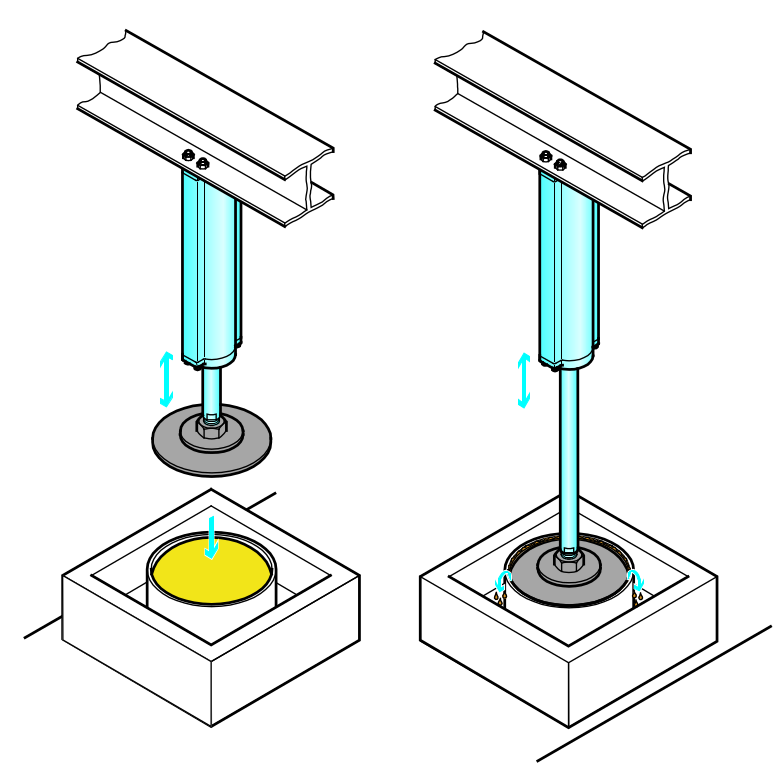
\includegraphics[width=6cm]{./cheese-stamping.png}};
  \node[coordinate] (cstart) at (-5,-4) {};
  \node[coordinate] (cstart2) at (-2.3,-4) {};
  \pgfmathsetmacro\sw{0.2}
  \pgfmathsetmacro\sd{0.5}
  \pgfmathsetmacro\slen{2}
  \pgfmathsetmacro\skew{0.3}
  \begin{scope}[rotate=30]
    \draw[fill=red!50] (cstart) -- ++(-\sw*\skew,\sw) -- ++(\slen, 0) -- ++ (\skew*2*\sw, -2*\sw) node[coordinate] (corner) {} -- ++ (-\slen, 0) -- cycle;
    \draw[fill=red!60] (cstart) ++(-\sw*\skew, \sw) -- ++(-0.5*\skew*\sd, -\skew*\sd) -- ++ (2*\sw*\skew, -2*\sw) -- ++(\slen, 0) -- (corner);
    \draw[fill=red!50] (cstart) -- ++(-\sw*\skew,\sw) -- ++(\slen, 0) -- ++ (\skew*2*\sw, -2*\sw) node[coordinate] (corner) {} -- ++ (-\slen, 0) -- cycle;
    \draw[double] ($(corner) + (-0.01, 0.1)$) -- ++(0.73*\slen, 0);
  \end{scope}
  \begin{scope}[rotate=30]
    \draw[] (cstart2) -- ++(-\sw*\skew,\sw) -- ++(\slen, 0) -- ++ (\skew*2*\sw, -2*\sw) node[coordinate] (corner) {} -- ++ (-\slen, 0) -- cycle;
    \draw[fill=red!60] (cstart2) ++(-\sw*\skew, \sw) -- ++(-0.5*\skew*\sd, -\skew*\sd) -- ++ (2*\sw*\skew, -2*\sw) -- ++(\slen, 0) -- (corner);
    \draw[fill=red!50] (cstart2) -- ++(-\sw*\skew,\sw) -- ++(\slen, 0) -- ++ (\skew*2*\sw, -2*\sw) node[coordinate] (corner) {} -- ++ (-\slen, 0) -- cycle;
    \draw[double] ($(corner) + (-0.01, 0.1)$) -- ++(0.74*\slen, 0);
  \end{scope}
  \node at ($(cstart) + (0,6mm)$) {\large  A};
  \node at (-2,1) {\large B};
\end{tikzpicture}
\end{document}
